%%%%%%%%%%%%%%%%%%%%%%%%%%%%%%%%%%%%%%%%%
% Beamer Presentation
% LaTeX Template
% Version 1.0 (10/11/12)
%
% This template has been downloaded from:
% http://www.LaTeXTemplates.com
%
% License:
% CC BY-NC-SA 3.0 (http://creativecommons.org/licenses/by-nc-sa/3.0/)
%
%%%%%%%%%%%%%%%%%%%%%%%%%%%%%%%%%%%%%%%%%

%----------------------------------------------------------------------------------------
%	PACKAGES AND THEMES
%----------------------------------------------------------------------------------------

\documentclass[UTF8,aspectratio=169,14pt]{ctexbeamer}

\usepackage{hyperref}
\hypersetup{
	colorlinks=true,
	linkcolor=red,
	anchorcolor=blue,
	citecolor=green
}

\mode<presentation> {
	
	% The Beamer class comes with a number of default slide themes
	% which change the colors and layouts of slides. Below this is a list
	% of all the themes, uncomment each in turn to see what they look like.
	
	%\usetheme{default}
	%\usetheme{AnnArbor}
	%\usetheme{Antibes}
	%\usetheme{Bergen}
	%\usetheme{Berkeley}
	%\usetheme{Berlin}
	%\usetheme{Boadilla}
	%\usetheme{CambridgeUS}
	%\usetheme{Copenhagen}
	%\usetheme{Darmstadt}
	%\usetheme{Dresden}
	%\usetheme{Frankfurt}
	%\usetheme{Goettingen}
	%\usetheme{Hannover}
	%\usetheme{Ilmenau}
	%\usetheme{JuanLesPins}
	%\usetheme{Luebeck}
	\usetheme{Madrid}
	%\usetheme{Malmoe}
	%\usetheme{Marburg}
	%\usetheme{Montpellier}
	%\usetheme{PaloAlto}
	%\usetheme{Pittsburgh}
	%\usetheme{Rochester}
	%\usetheme{Singapore}
	%\usetheme{Szeged}
	%\usetheme{Warsaw}
	
	% As well as themes, the Beamer class has a number of color themes
	% for any slide theme. Uncomment each of these in turn to see how it
	% changes the colors of your current slide theme.
	
	%\usecolortheme{albatross}
	%\usecolortheme{beaver}
	%\usecolortheme{beetle}
	%\usecolortheme{crane}
	%\usecolortheme{dolphin}
	%\usecolortheme{dove}
	%\usecolortheme{fly}
	%\usecolortheme{lily}
	%\usecolortheme{orchid}
	%\usecolortheme{rose}
	%\usecolortheme{seagull}
	%\usecolortheme{seahorse}
	%\usecolortheme{whale}
	%\usecolortheme{wolverine}
	
	%\setbeamertemplate{footline} % To remove the footer line in all slides uncomment this line
	%\setbeamertemplate{footline}[page number] % To replace the footer line in all slides with a simple slide count uncomment this line
	
	%\setbeamertemplate{navigation symbols}{} % To remove the navigation symbols from the bottom of all slides uncomment this line
}

\usepackage{graphicx} % Allows including images
\graphicspath{{./figs/}}
\usepackage{booktabs} % Allows the use of \toprule, \midrule and \bottomrule in tables
\usepackage{longtable}
\usepackage{listings}
\usepackage{xcolor}
\lstset{numbers=left, %设置行号位置
	numberstyle=\tiny, %设置行号大小
	keywordstyle=\color{blue}, %设置关键字颜色
	commentstyle=\color[cmyk]{1,0,1,0}, %设置注释颜色
	frame=single, %设置边框格式
	escapeinside=``, %逃逸字符(1左面的键),用于显示中文
	%breaklines, %自动折行
	extendedchars=false, %解决代码跨页时,章节标题,页眉等汉字不显示的问题
	xleftmargin=2em,xrightmargin=2em, aboveskip=1em, %设置边距
	tabsize=4, %设置tab空格数
	showspaces=false %不显示空格
}
% Fonts
% \usepackage{libertine}
% \setmonofont{Courier}
\setCJKsansfont[ItalicFont=Noto Serif CJK SC Black, BoldFont=Noto Sans CJK SC Black]{Noto Sans CJK SC}

%\def\imagepath{./resources/graphics}
%\usepackage[imagepath=\imagepath]{ditaa}
%\graphicspath{ {\imagepath/} }


%\usepackage{pgfpages}
%\setbeameroption{show notes on second screen}
%%----------------------------------------------------------------------------------------
%	TITLE PAGE
%----------------------------------------------------------------------------------------

\title[第8讲]{第8讲 :全局页替换算法} % The short title appears at the bottom of every slide, the full title is only on the title page
\subtitle{第四节:面向缓存的页替换算法 -- LIRS}
\author{向勇、陈渝、李国良} % Your name
\institute[清华大学] % Your institution as it will appear on the bottom of every slide, may be shorthand to save space
{
	清华大学计算机系 \\ % Your institution for the title page
	\medskip
	\textit{xyong,yuchen,liguoliang@tsinghua.edu.cn} % Your email address
}
\date{\today} % Date, can be changed to a custom date


\begin{document}

\begin{frame}
\titlepage % Print the title page as the first slide
\end{frame}

%\begin{frame}
%\frametitle{提纲} % Table of contents slide, comment this block out to remove it
%\tableofcontents % Throughout your presentation, if you choose to use \section{} and \subsection{} commands, these will automatically be printed on this slide as an overview of your presentation
%\end{frame}
%
%%----------------------------------------------------------------------------------------
%%	PRESENTATION SLIDES
%%----------------------------------------------------------------------------------------
%2002 LIRS : An Efficient Replacement Policy to Improve Buffer Cache Performance 
% ppt from Song Jiang1 and Xiaodong Zhang1,2
%----------------------------------------------
\begin{frame}[plain]
	\frametitle{ }
	\begin{columns}
		\begin{column}{.5\textwidth}
			\centering
			%			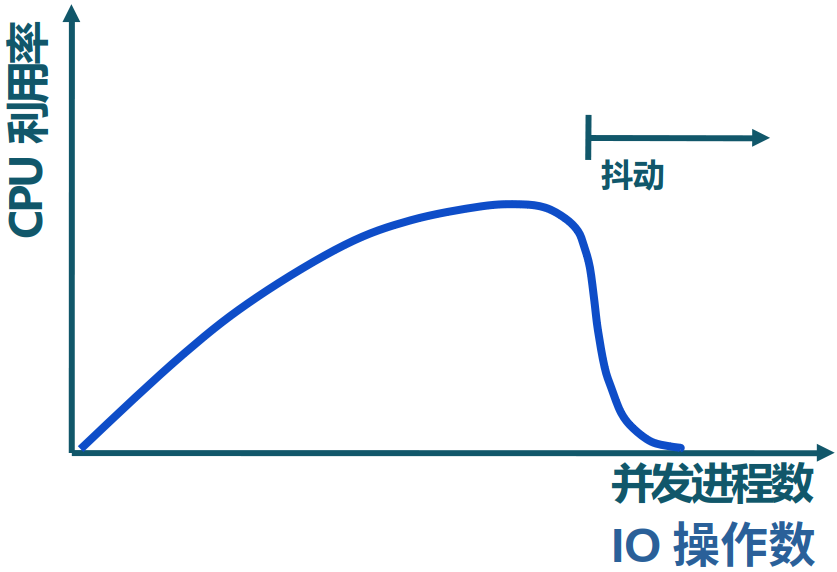
\includegraphics[width=.6\textwidth]{mem-trash}
			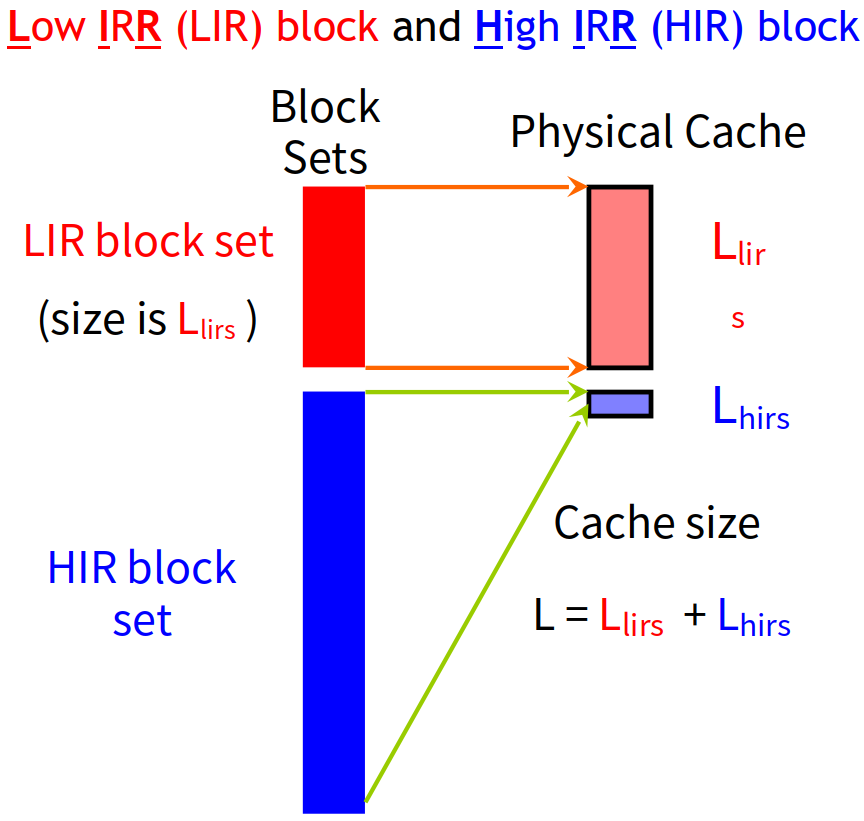
\includegraphics[width=1.\textwidth]{lirs}
			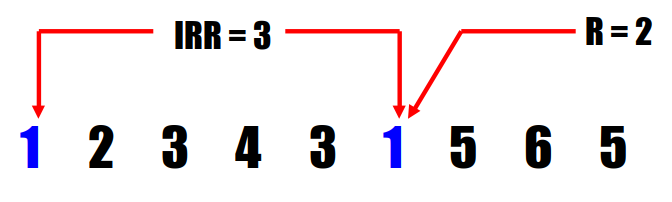
\includegraphics[width=.5\textwidth]{lirs-irr-r}
		\end{column}
		
		\begin{column}{.5\textwidth}
			LIRS (Low Inter-reference Recency Set)\textbf{}
%			\begin{itemize}
				
				\begin{itemize}
					\item Recency:最近被访问的不重复块数(表示时间属性)。
					\item IRR(Inter-Reference Recency ):同一块连续两次访问期间中间访问过的不重复块数。
					\item  LIRS算法动态区分低IRR(LIR)和高IRR(HIR)的块,LIR块一般会常驻cache,HIR块则会较快被替换出cache。
					\item 基本思路:如果块的IRR值高,那么它的下一次IRR值也会很高,所以要替换IRR值高的块。
%					\item 要保证所有LIR块都能缓存,只有比例较小的Cache供HIR块缓存,当LIR块的Recency超过某个值,且HIR块在一个更小的Recency中被访问,两者的状态就会交换。

					
				\end{itemize}
%			\end{itemize}
%			\centering
			\tiny LIRS: An Efficient Low Inter-reference Recency Set Replacement Policy to Improve Buffer Cache Performance, Song Jiang, Xiaodong Zhang, SIGMETRICS, 2002
			
		\end{column}
		
		
	\end{columns}
\end{frame}


%----------------------------------------------
\begin{frame}[plain]
	\frametitle{ }
	\begin{columns}
		\begin{column}{.4\textwidth}
			\centering
			%			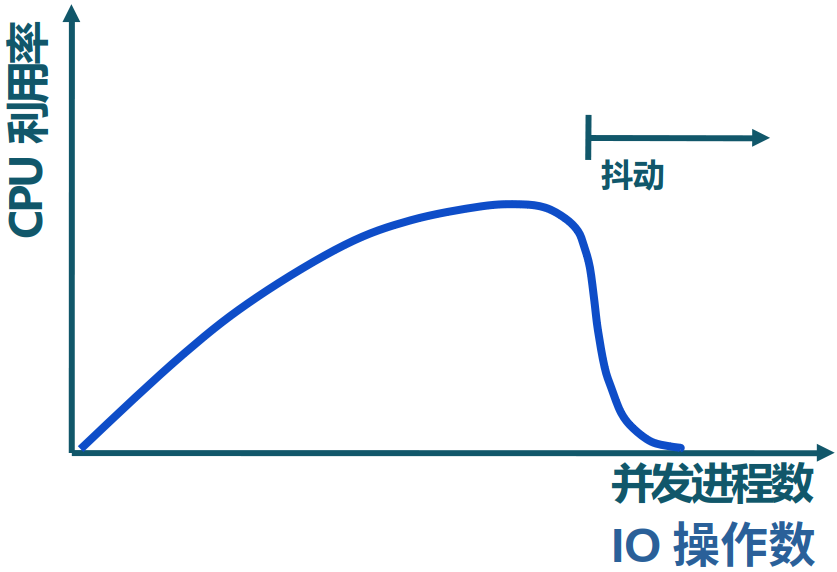
\includegraphics[width=.6\textwidth]{mem-trash}
				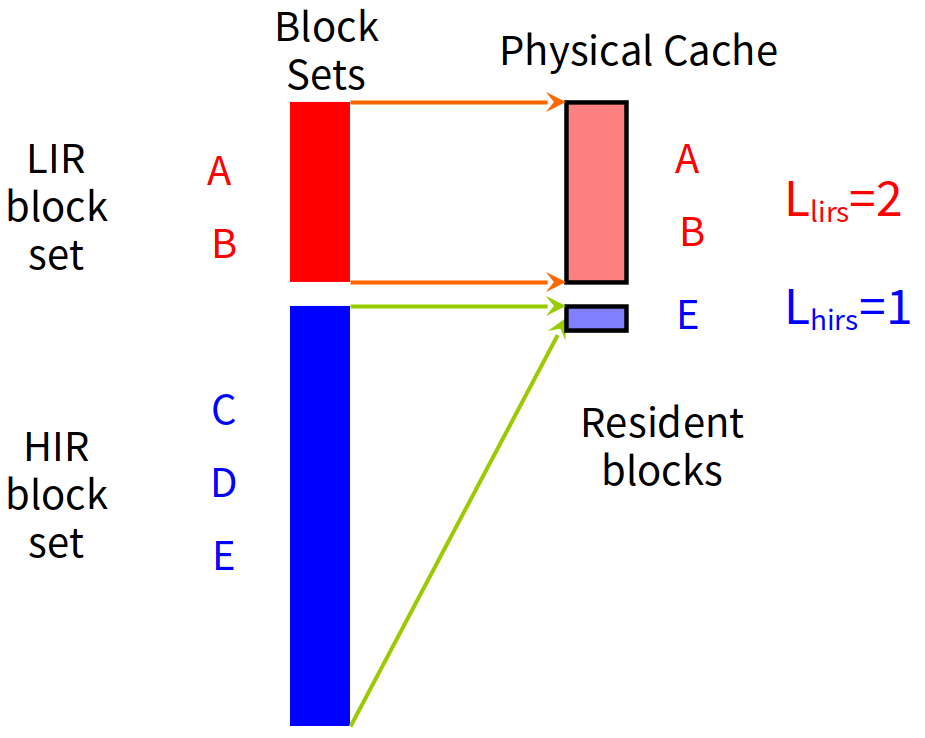
\includegraphics[width=1.\textwidth]{lirs-ex-map}
		\end{column}
		
		\begin{column}{.6\textwidth}
			LIRS 例子
			
		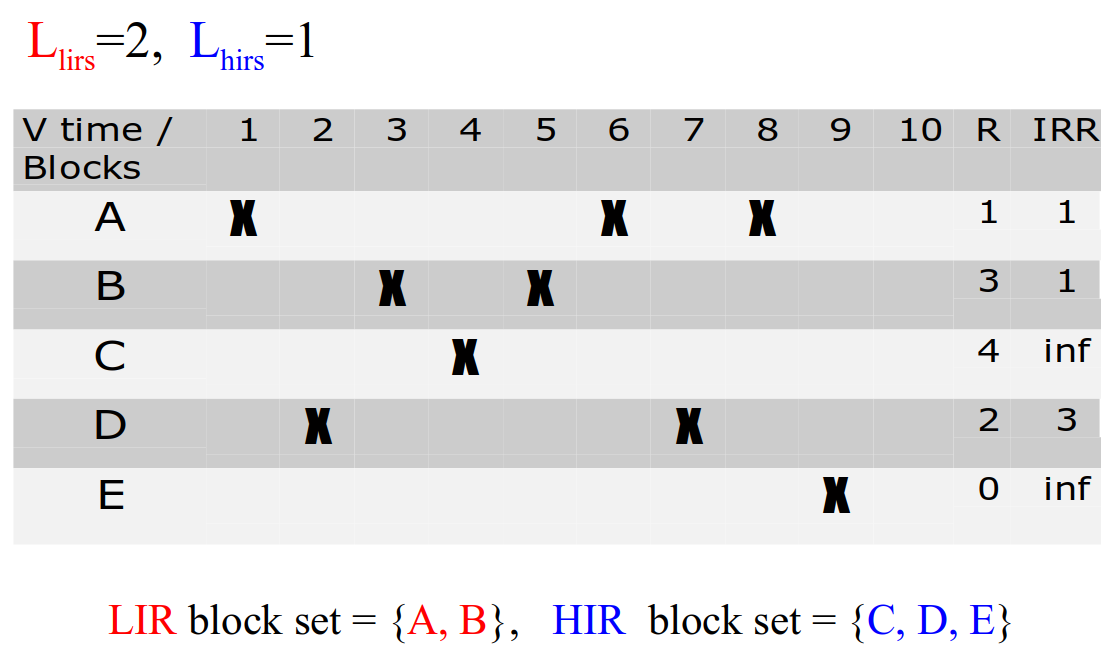
\includegraphics[width=1.\textwidth]{lirs-example}
			
		\end{column}
		
		
	\end{columns}
\end{frame}


%----------------------------------------------
\begin{frame}[plain]
	\frametitle{ }
	\begin{columns}
		\begin{column}{.4\textwidth}
			\centering
			%			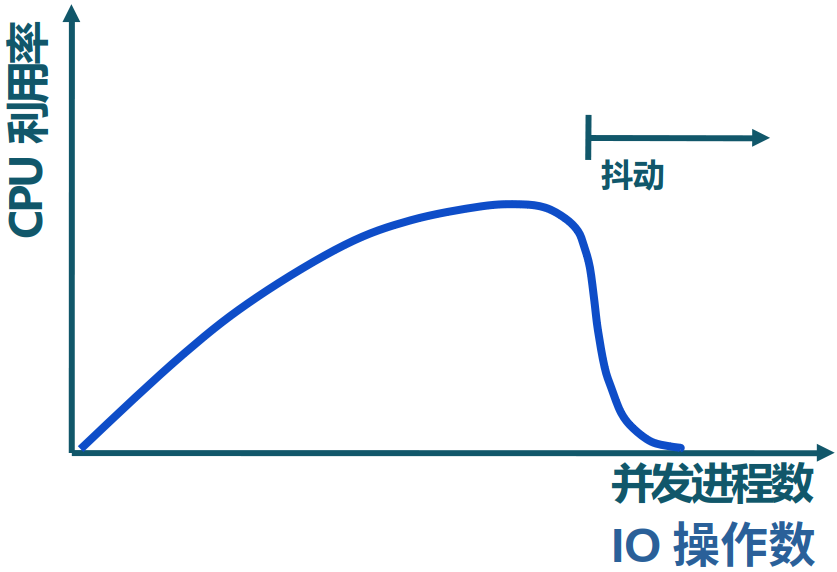
\includegraphics[width=.6\textwidth]{mem-trash}
%			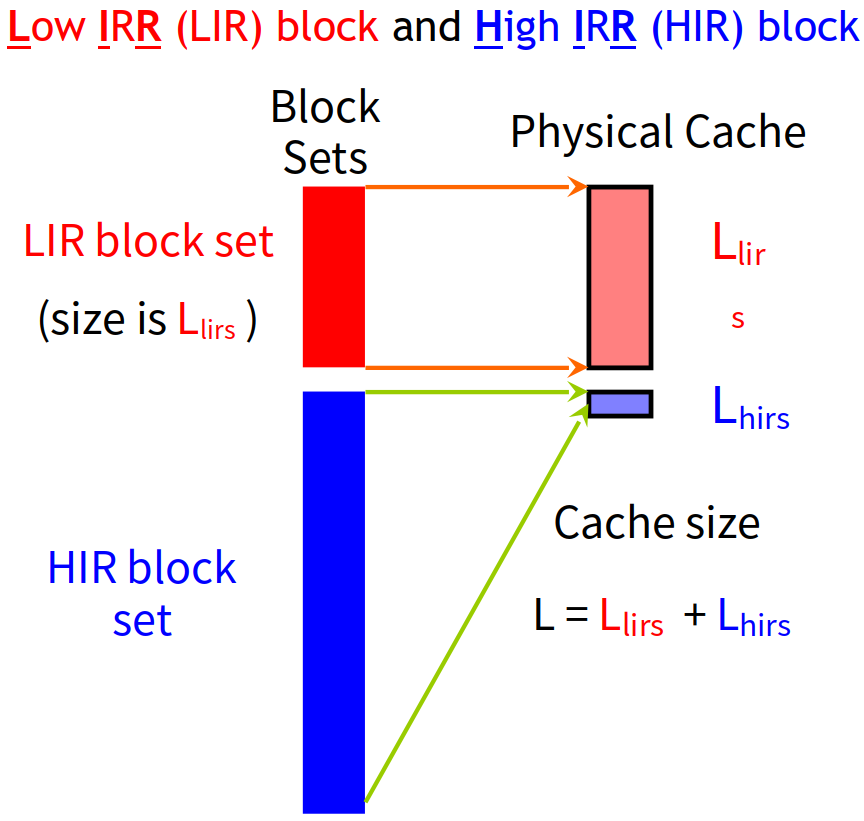
\includegraphics[width=1.\textwidth]{lirs}
			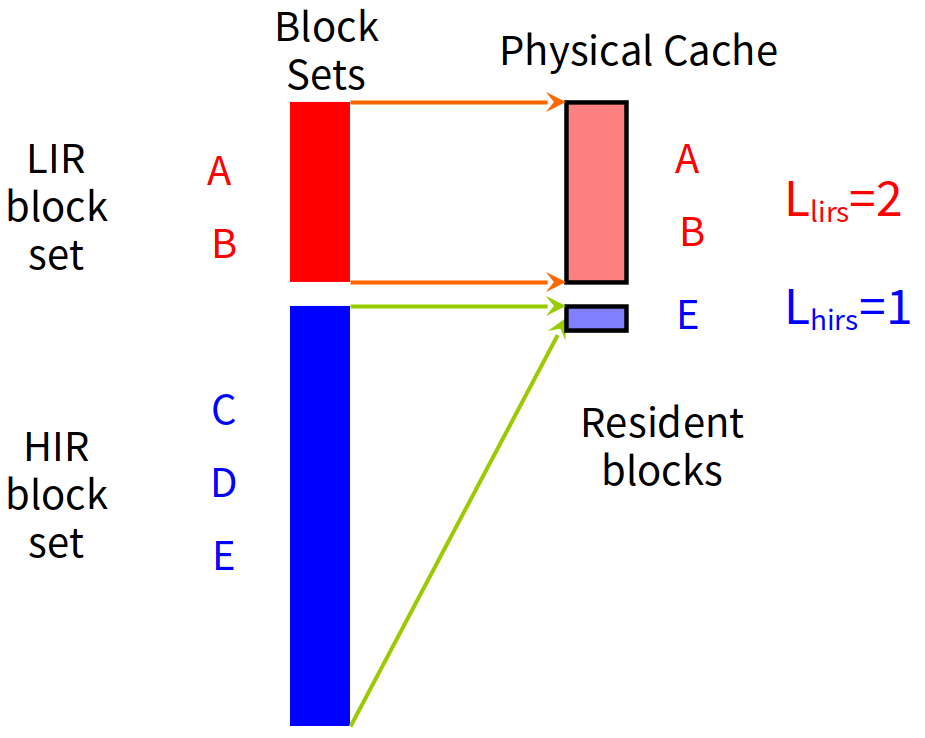
\includegraphics[width=1.\textwidth]{lirs-ex-map}
		\end{column}
		
		\begin{column}{.6\textwidth}
			LIRS 例子:D在时刻10被访问,替换哪个块?
			
			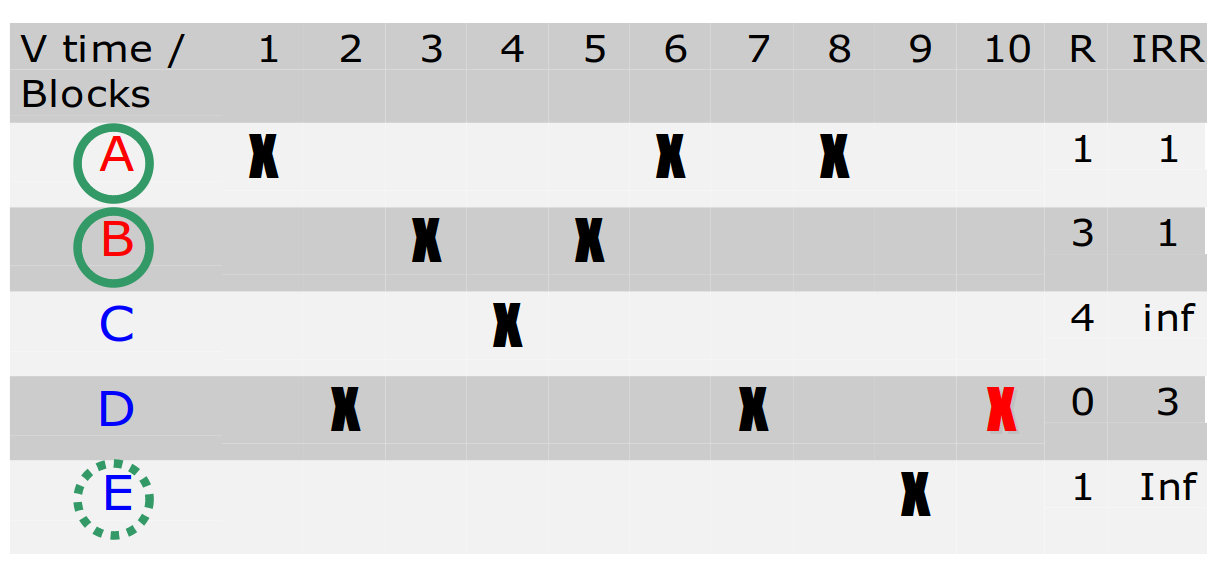
\includegraphics[width=1.\textwidth]{lirs-ex2}
			\pause
			\centering
			替换 HIR块 E	
		\end{column}
		
		
	\end{columns}
\end{frame}




%----------------------------------------------
\begin{frame}[plain]
	\frametitle{ }
	\begin{columns}
		\begin{column}{.4\textwidth}
			\centering
			%			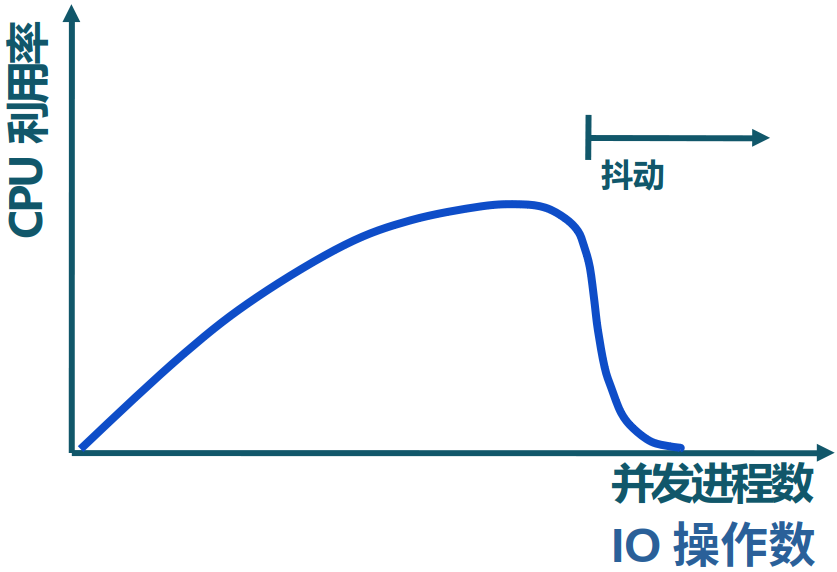
\includegraphics[width=.6\textwidth]{mem-trash}
			%			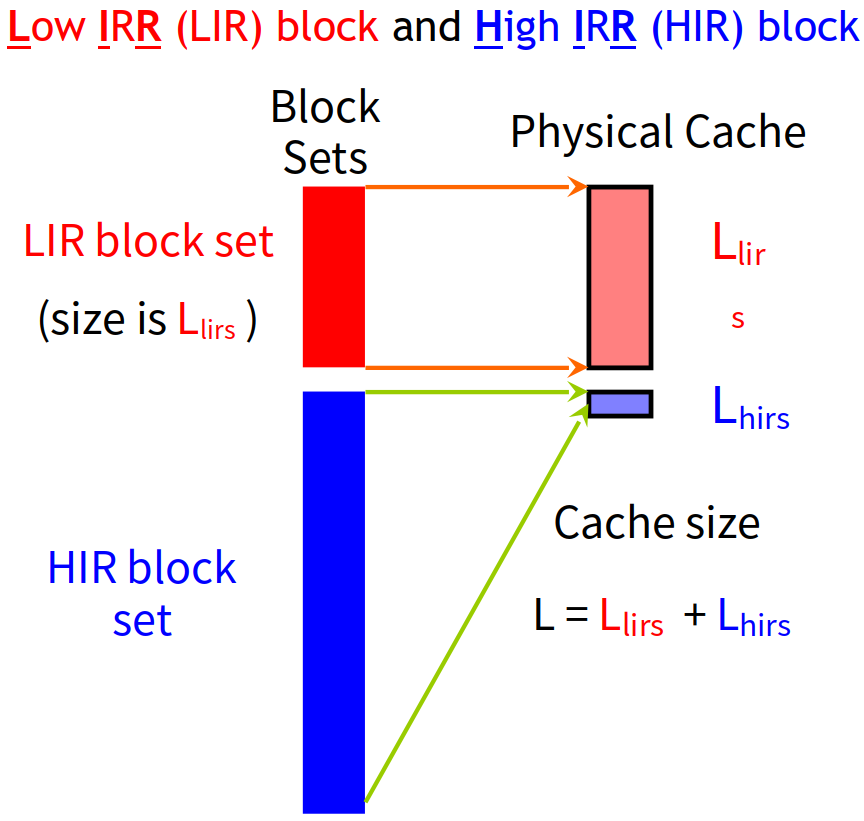
\includegraphics[width=1.\textwidth]{lirs}
			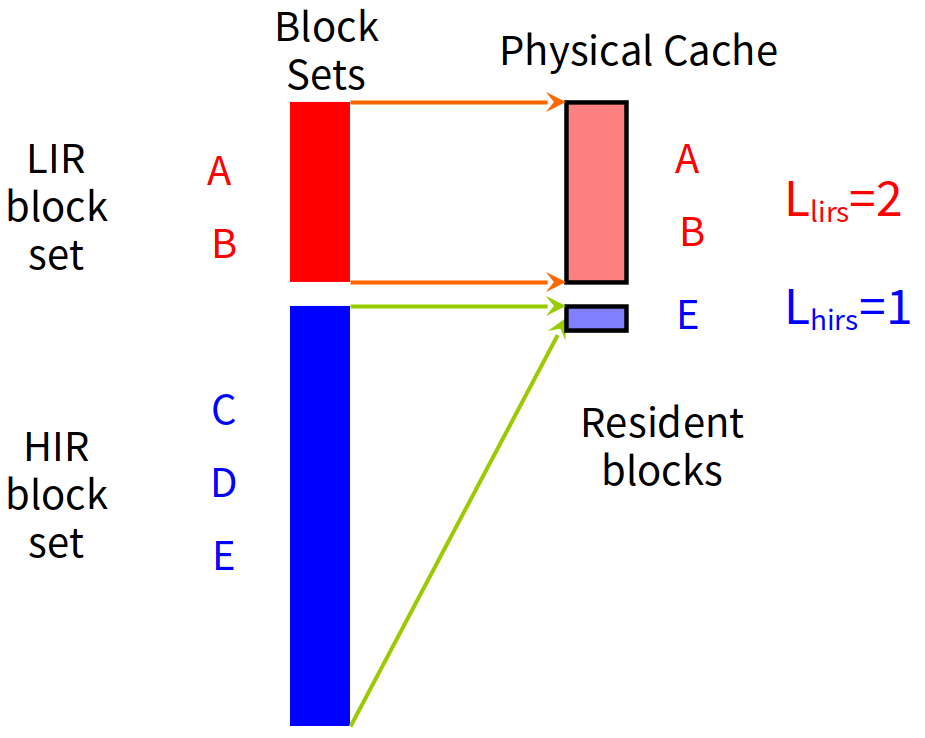
\includegraphics[width=1.\textwidth]{lirs-ex-map}
		\end{column}
		
		\begin{column}{.6\textwidth}
			LIRS 例子:LIR Set如何更新?
			
			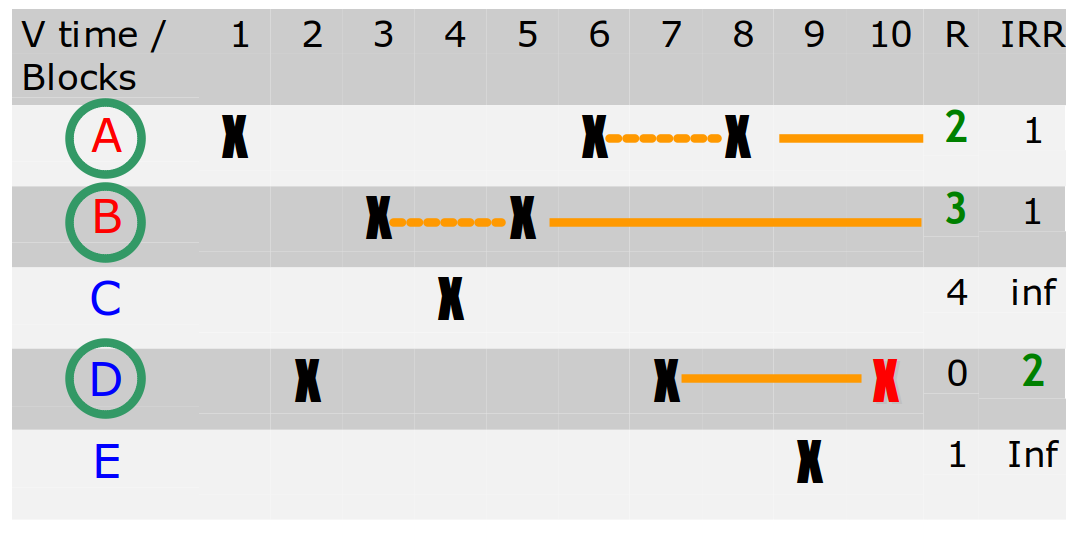
\includegraphics[width=1.\textwidth]{lirs-ex3}
			

		\end{column}
		
		
	\end{columns}
\end{frame}


%----------------------------------------------
\begin{frame}[plain]
	\frametitle{ }
	\begin{columns}
		\begin{column}{.4\textwidth}
			\centering
			%			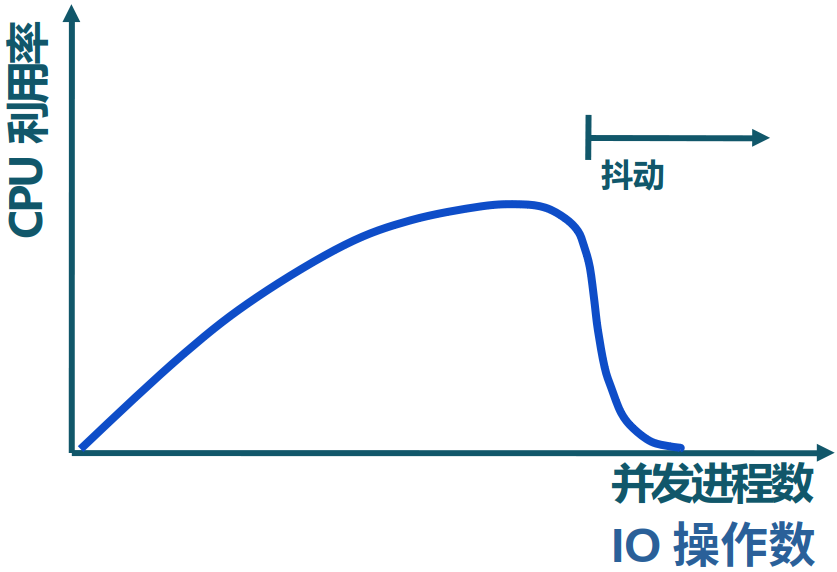
\includegraphics[width=.6\textwidth]{mem-trash}
			%			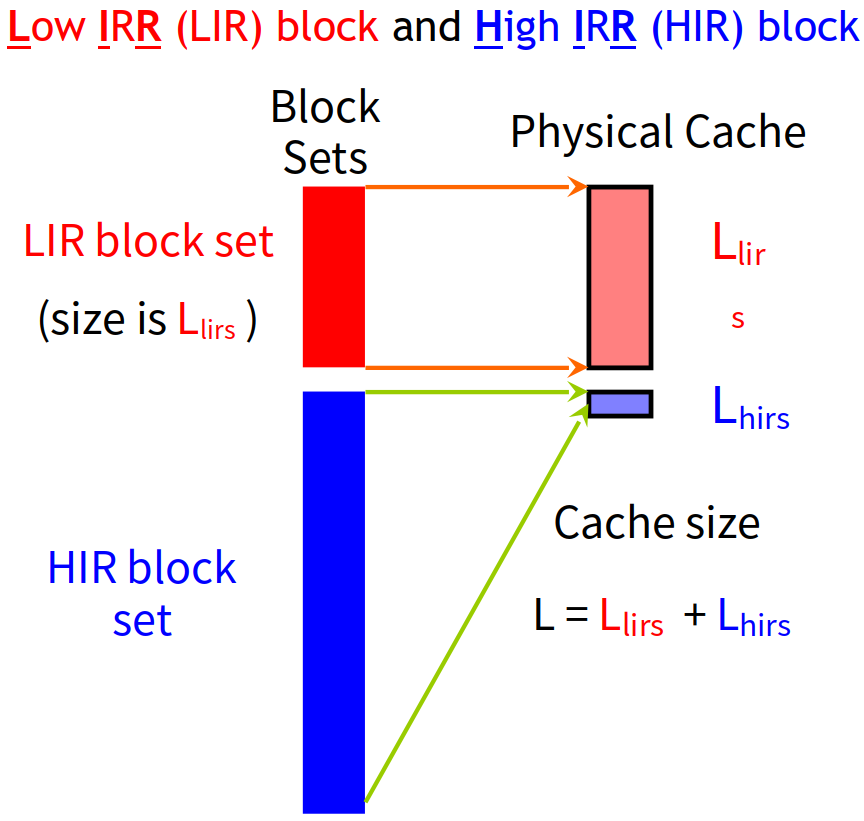
\includegraphics[width=1.\textwidth]{lirs}
			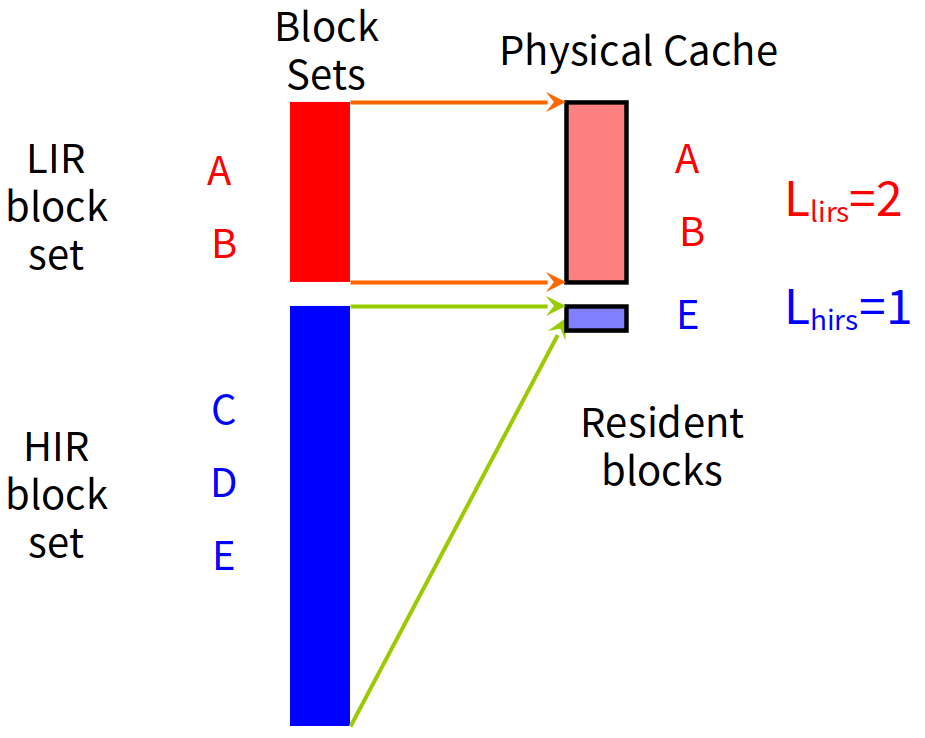
\includegraphics[width=1.\textwidth]{lirs-ex-map}
		\end{column}
		
		\begin{column}{.6\textwidth}
			LIRS 例子:LIR Set如何更新?
			
			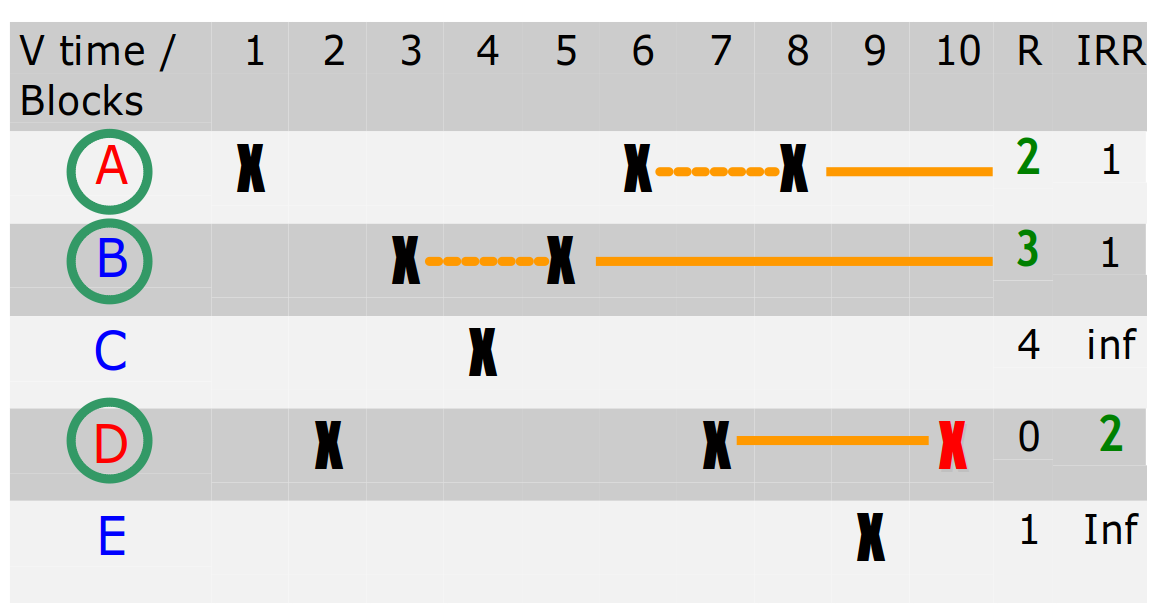
\includegraphics[width=1.\textwidth]{lirs-ex4}
			
			E被替换,D进入LIR Set,B进入HIR Set 
		\end{column}
		
		
	\end{columns}
\end{frame}


%----------------------------------------------
\begin{frame}[plain]
	\frametitle{ }
	\begin{columns}
		\begin{column}{.4\textwidth}
			\centering
			%			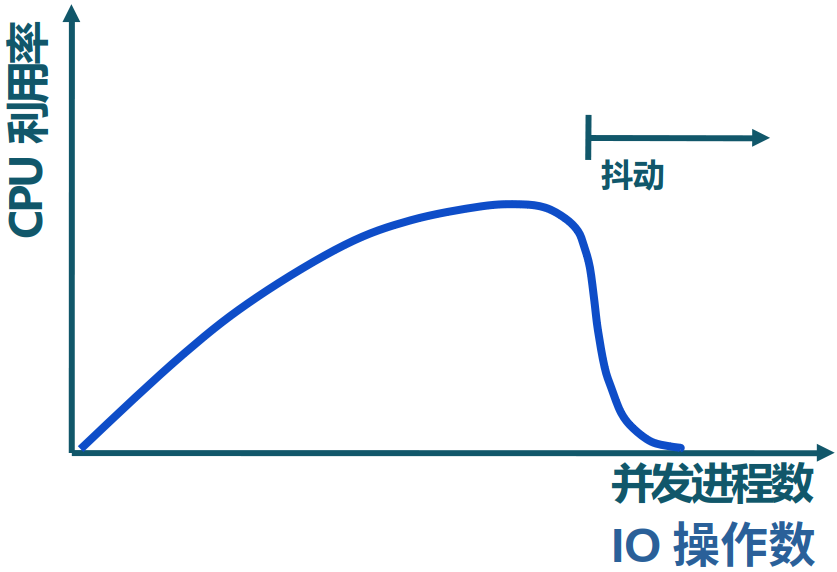
\includegraphics[width=.6\textwidth]{mem-trash}
			%			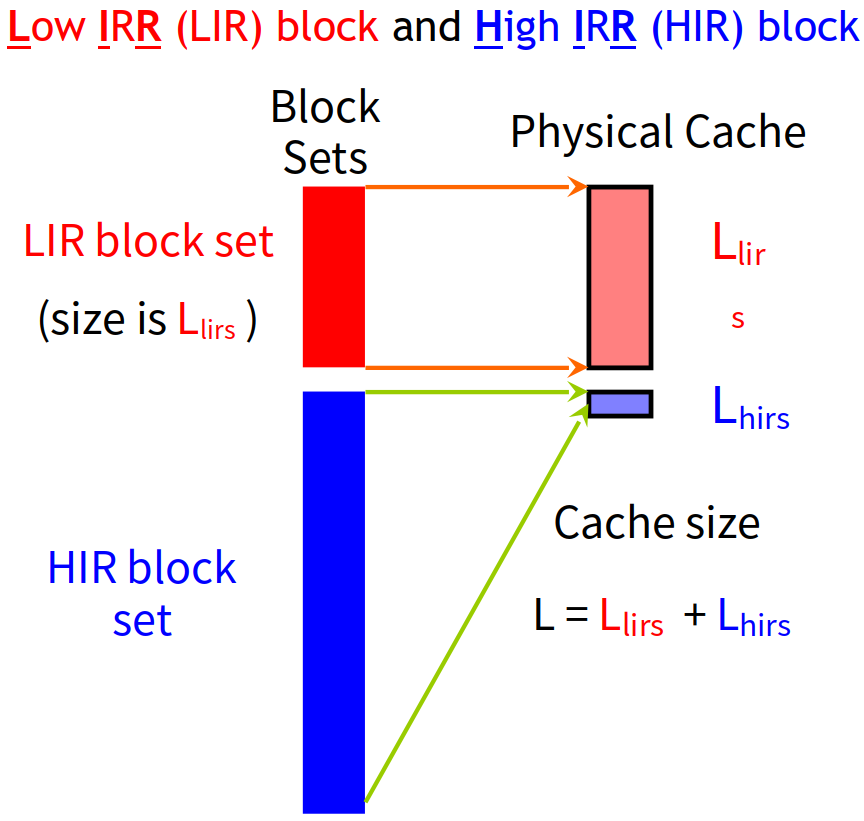
\includegraphics[width=1.\textwidth]{lirs}
			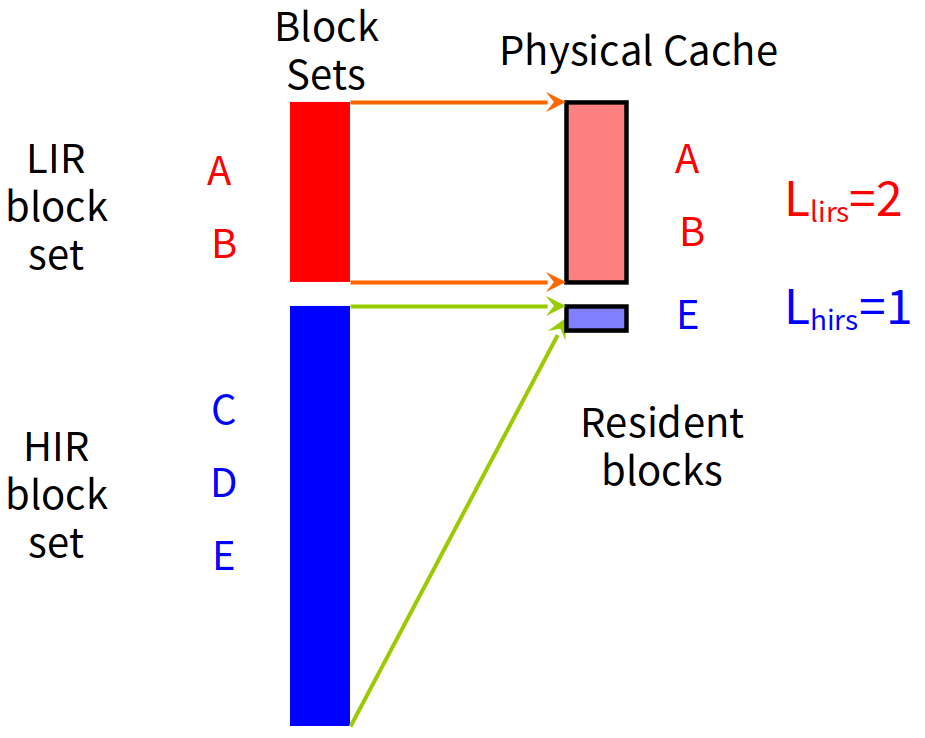
\includegraphics[width=1.\textwidth]{lirs-ex-map}
		\end{column}
		
		\begin{column}{.6\textwidth}
			LIRS 例子:C在时刻10被访问,替换哪个块?如何更新LIR/HIR Set?
			
			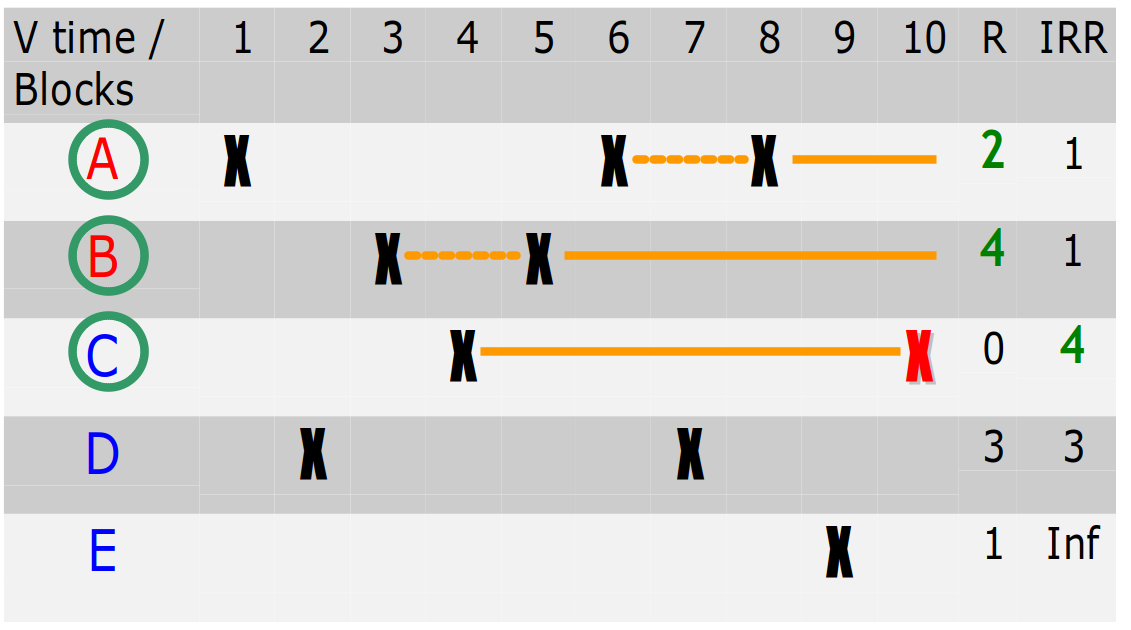
\includegraphics[width=1.\textwidth]{lirs-ex5}
			
			\pause
			\centering
			E被替换,C不能进入LIR块集合 
		\end{column}
		
		
	\end{columns}
\end{frame}


%----------------------------------------------
\begin{frame}[plain]
	\frametitle{ }
	\begin{columns}
		\begin{column}{.5\textwidth}
			\centering
			%			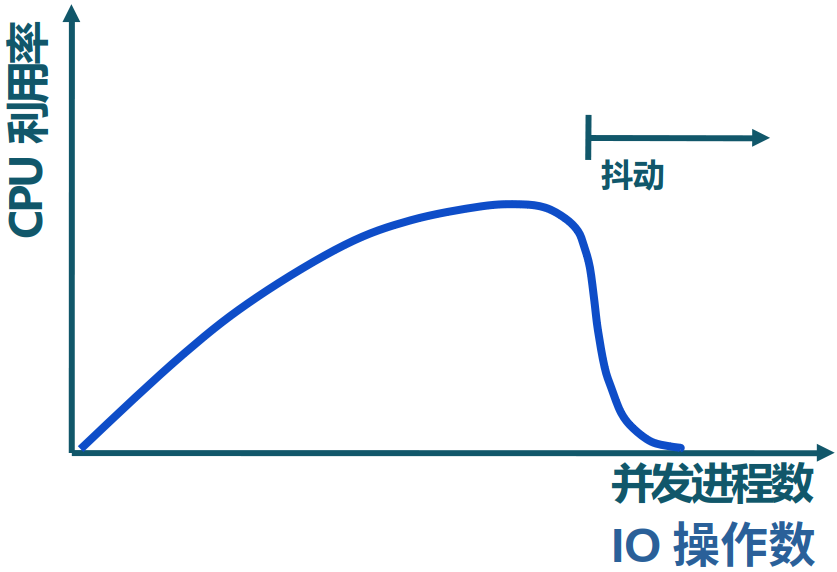
\includegraphics[width=.6\textwidth]{mem-trash}
			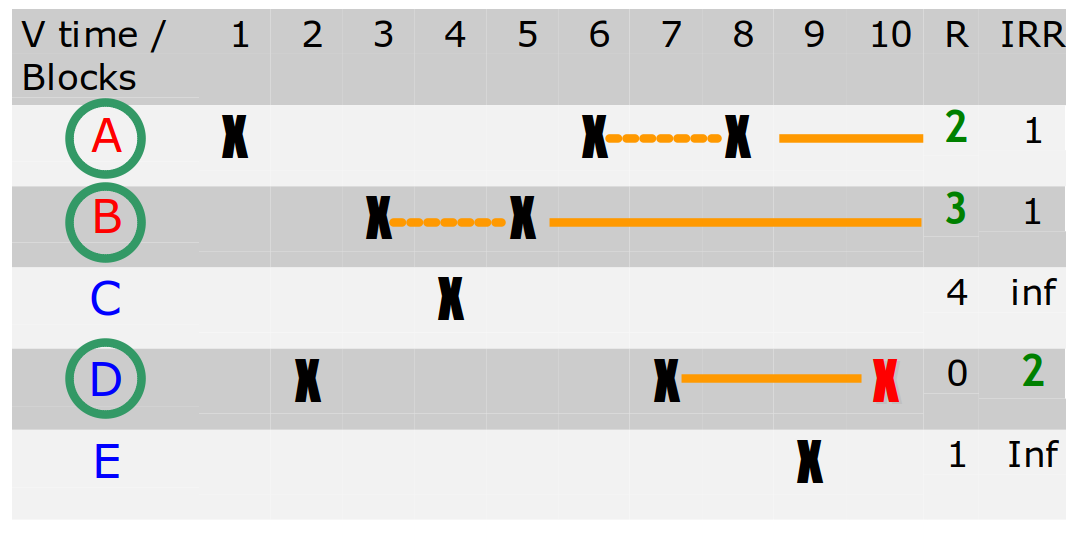
\includegraphics[width=.8\textwidth]{lirs-ex3}
			
			E被换掉,D与B的状态进行了交换 
			
			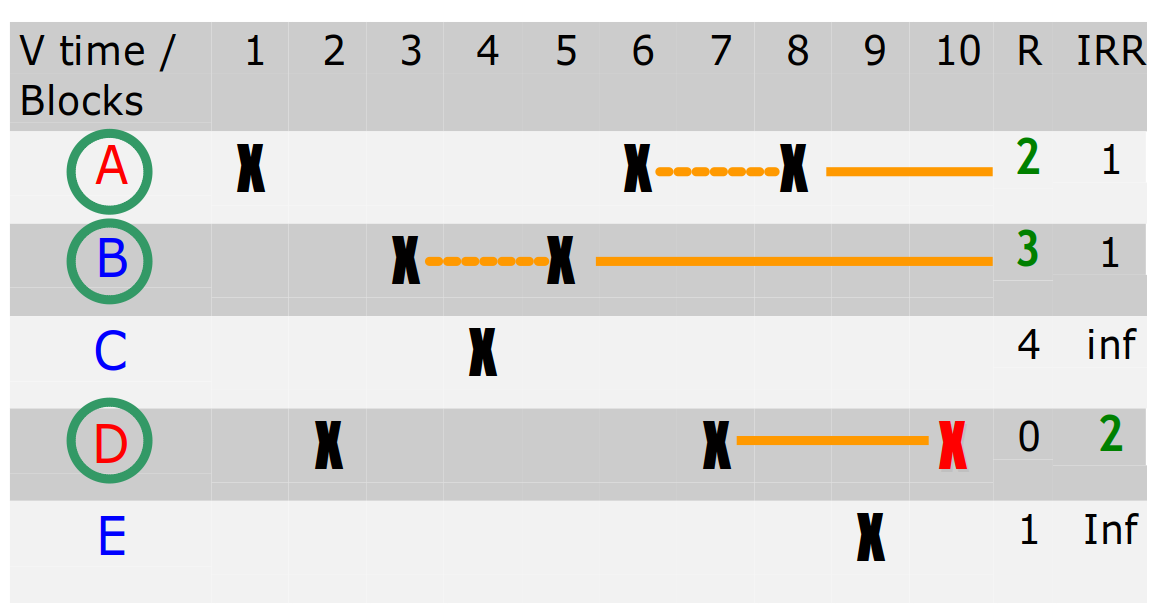
\includegraphics[width=.8\textwidth]{lirs-ex4}
		\end{column}
		
		\begin{column}{.5\textwidth}
			LIRS 替换策略
			%			\begin{itemize}
			
			\begin{itemize}

				\item  LIR块一般会常驻cache,HIR块则会较快被替换出cache。通常假设LIR占99\%的cache大小,HIR占1\%即可。 
				\item 如果块的IRR值高,那么它的下一次IRR值也会很高,所以要替换IRR值高的块。
				\item 要保证所有LIR块都能缓存,当LIR块的Recency超过IRR最大值,且HIR块在一个更小的Recency中被访问,两者的状态就会交换。
				
				
			\end{itemize}
			%			\end{itemize}
			%			\centering
			%			\large 从能否进一步改进?
			
		\end{column}
		
		
	\end{columns}
\end{frame}




%----------------------------------------------
\begin{frame}[plain]
	\frametitle{ }
	\begin{columns}
		\begin{column}{.5\textwidth}
			\centering
			%			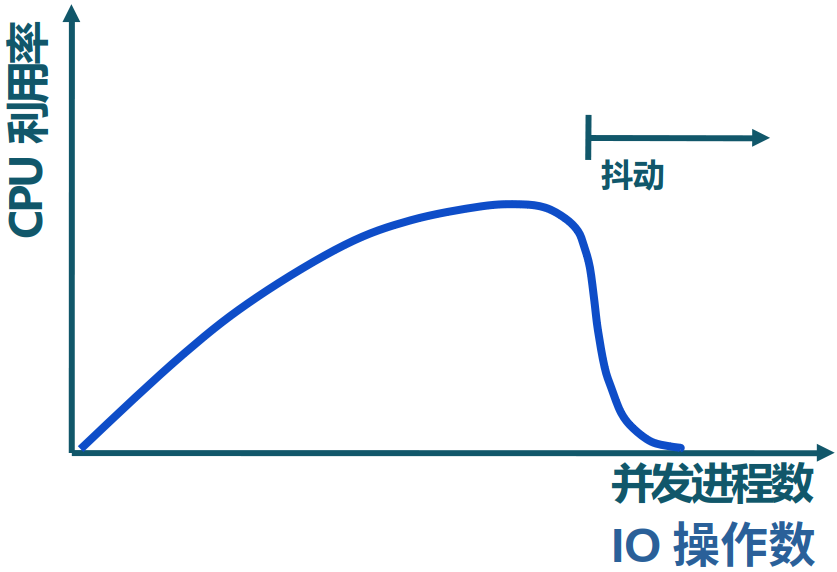
\includegraphics[width=.6\textwidth]{mem-trash}
			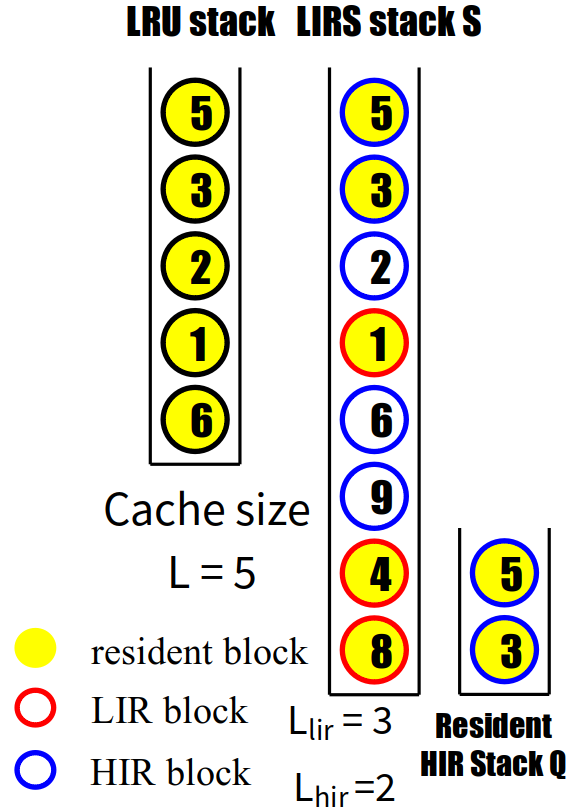
\includegraphics[width=.8\textwidth]{lirs-stack}
			
		\end{column}
		
		\begin{column}{.5\textwidth}
			LIRS 替换算法
			%			\begin{itemize}
			
			\begin{itemize}
				\item Stack S:  包括LIR块、少于LIR块最大recency的HIR块
				\item Stack Q:  HIR块FIFO缓存队列(加快HIR块缓存的搜索)

				\item “栈裁剪”操作,栈S的底部LIR块被删除,则一直删除底部块直到遇到另一个LIR块。这样做的目的是因为如果底部存在HIR块,则这些HIR块必定大于LIR块的最大recency,这样它们肯定不能转变为LIR块。
				
				
			\end{itemize}
			%			\end{itemize}
			%			\centering
			%			\large 从能否进一步改进?
			
		\end{column}
		
		
	\end{columns}
\end{frame}


%----------------------------------------------
\begin{frame}[plain]
	\frametitle{ }
	\begin{columns}
		\begin{column}{.1\textwidth}
			\centering
			%			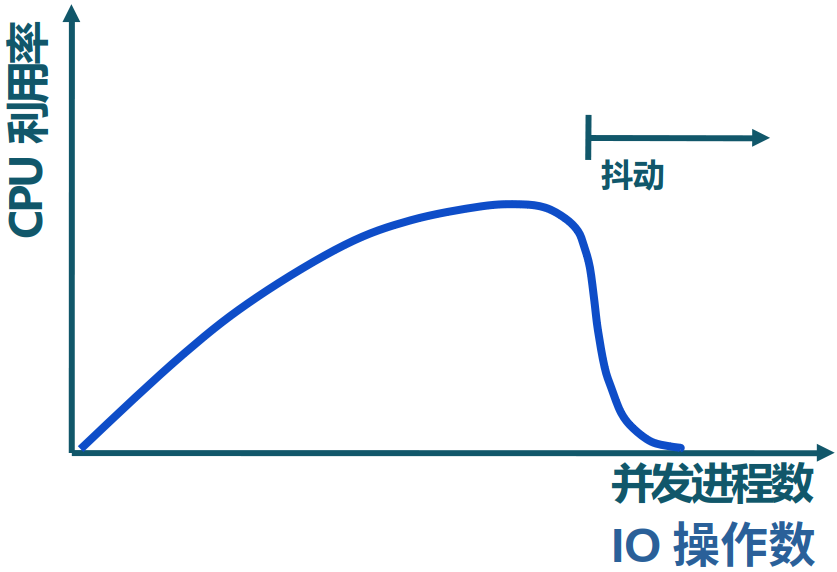
\includegraphics[width=.6\textwidth]{mem-trash}
%			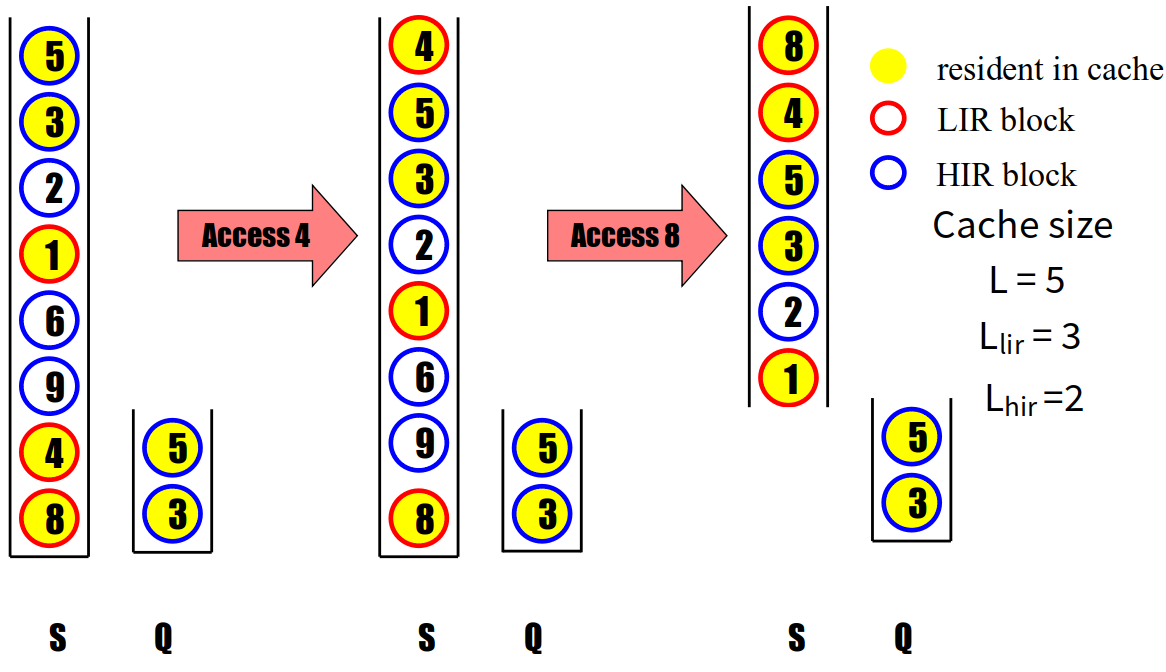
\includegraphics[width=.8\textwidth]{lirs-stack-hit}
			
		\end{column}
		
		\begin{column}{.9\textwidth}
			LIRS 替换算法 (LIR hit)
			%			\begin{itemize}
			
			\begin{itemize}
				\item 访问栈S中的LIR块X:LIR块必定驻cache中,所以必定命中缓存。然后把块X移动到栈S的头部,如果块X之前是在栈S的底部,则执行“栈裁剪”操作。
				
%				\item 访问驻cache中的HIR块X:访问命中缓存。把X移动到栈S头部。另外块X有两种情况:(1)块X在栈S中,把它状态转换为LIR,还删除队列Q中块X的cache。然后把栈S底部的LIR块转换为HIR块,然后移动到队列Q中。最后“栈裁剪”。(2)块X不在栈S中,则块X的状态保持HIR不变,然后从队列Q的cache移动到队列尾部。
%				
%				\item 访问非驻cache中的HIR块X:没有命中缓存。首先删除队列Q头部的HIR块(如果该块在栈S,则变为非驻cache状态),这样多出cache空间,然后加载块X到该cache空间,然后移动到栈S的顶部。块X同样有两种情况:(1)块X在栈S中,改变状态为LIR,并同时改变栈底部的LIR块为HIR块,并移动到队列Q的尾部,然后“栈裁剪”。(2)块X不在栈S中,则状态为HIR,并放到队列Q的尾部。
			
				
				
			\end{itemize}
			\centering
             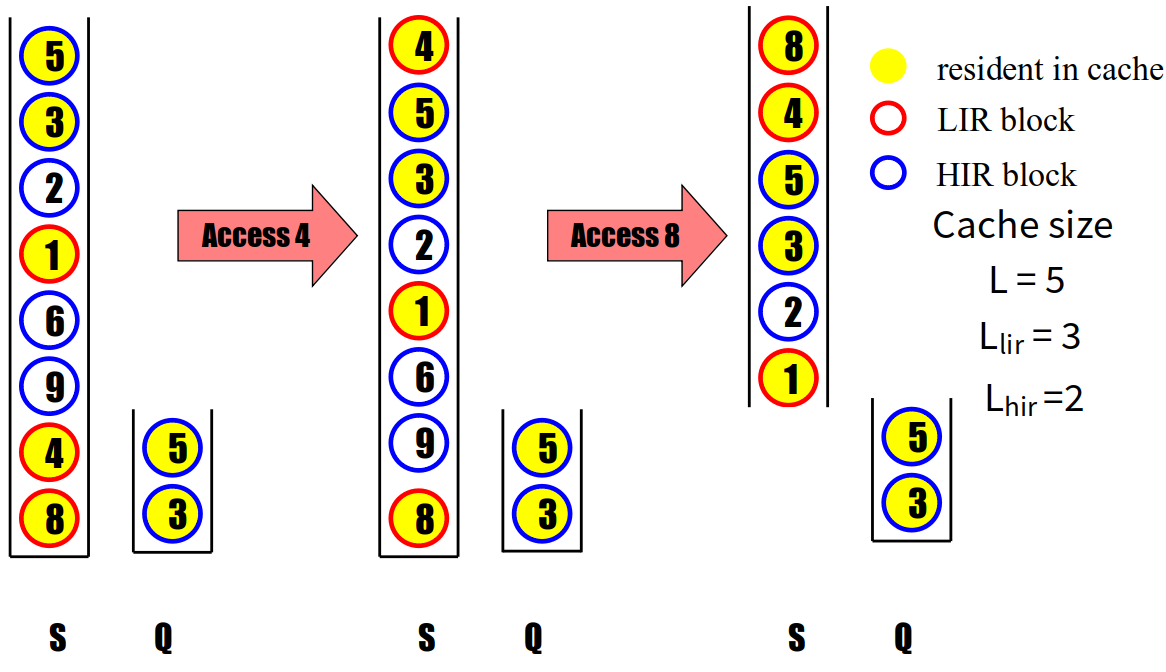
\includegraphics[width=.8\textwidth]{lirs-stack-hit}
			
		\end{column}
		
		
	\end{columns}
从\end{frame}


%----------------------------------------------
\begin{frame}[plain]
	\frametitle{ }
	\begin{columns}
		\begin{column}{.1\textwidth}
			\centering
			%			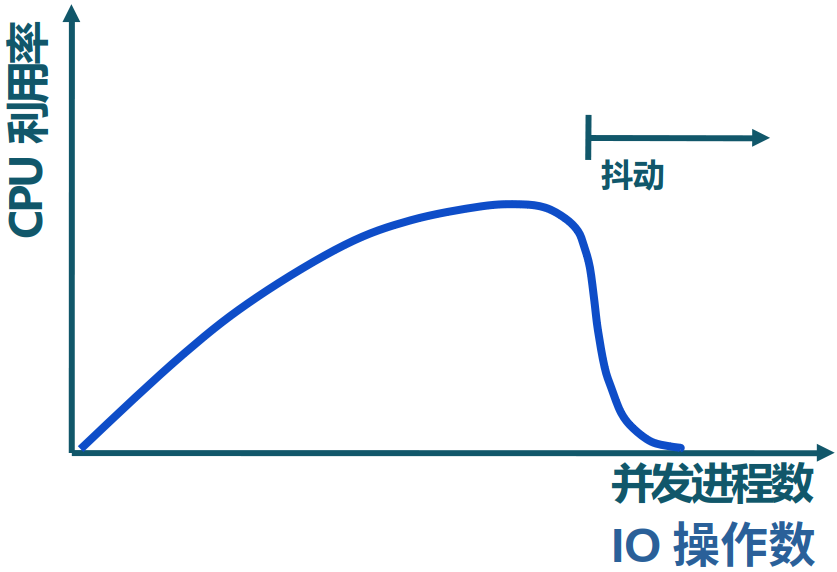
\includegraphics[width=.6\textwidth]{mem-trash}

			
		\end{column}
		
		\begin{column}{.9\textwidth}
			LIRS 替换算法 (HIR hit)
			%			\begin{itemize}
			
			\begin{itemize}
%				\item 访问栈S中的LIR块X:LIR块必定驻cache中,所以必定命中缓存。然后把块X移动到栈S的头部,如果块X之前是在栈S的底部,则执行“栈裁剪”操作。
				
			\item 访问驻cache中的HIR块X,把X移动到栈S头部,有两种情况:
%			\begin{itemize}
				\item 在S中,X状态转换为LIR,删除Q中X的cache,把S底部的LIR块转为HIR块,移动到Q中,最后“栈裁剪”。
				\item 不在S中,则X状态保持HIR,从队列Q中移动到Q头部。
				%				
				%				\item 访问非驻cache中的HIR块X:没有命中缓存。首先删除队列Q头部的HIR块(如果该块在栈S,则变为非驻cache状态),这样多出cache空间,然后加载块X到该cache空间,然后移动到栈S的顶部。块X同样有两种情况:(1)块X在栈S中,改变状态为LIR,并同时改变栈底部的LIR块为HIR块,并移动到队列Q的尾部,然后“栈裁剪”。(2)块X不在栈S中,则状态为HIR,并放到队列Q的尾部。
				
%			\end{itemize}	
				
			\end{itemize}
			\centering
			 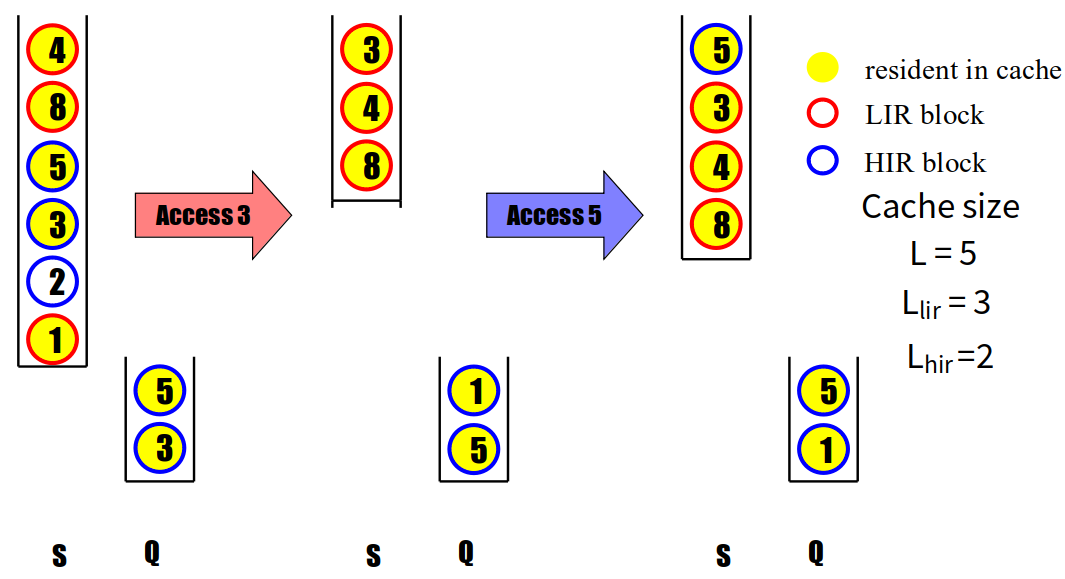
\includegraphics[width=.8\textwidth]{lirs-stack-hir-hit}
			
		\end{column}
		
		
	\end{columns}
\end{frame}




%----------------------------------------------
\begin{frame}[plain]
	\frametitle{ }
	\begin{columns}
		\begin{column}{.1\textwidth}
			\centering
			%			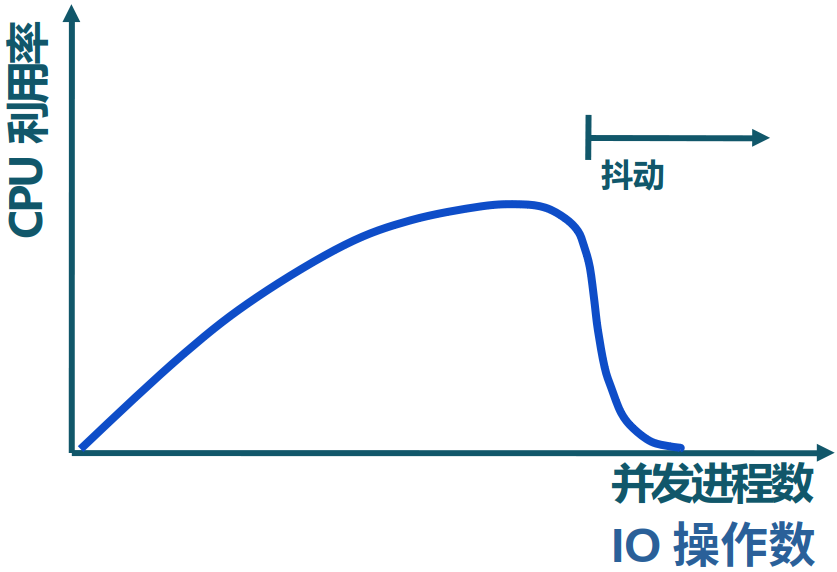
\includegraphics[width=.6\textwidth]{mem-trash}
			
			
		\end{column}
		
		\begin{column}{.9\textwidth}
			LIRS 替换算法 (Missing)
			%			\begin{itemize}
			
			\begin{itemize}
%				\item 访问栈S中的LIR块X:LIR块必定驻cache中,所以必定命中缓存。然后把块X移动到栈S的头部,如果块X之前是在栈S的底部,则执行“栈裁剪”操作。
				
%								\item 访问驻cache中的HIR块X:访问命中缓存。把X移动到栈S头部。另外块X有两种情况:(1)块X在栈S中,把它状态转换为LIR,还删除队列Q中块X的cache。然后把栈S底部的LIR块转换为HIR块,然后移动到队列Q中。最后“栈裁剪”。(2)块X不在栈S中,则块X的状态保持HIR不变,然后从队列Q的cache移动到队列尾部。
				%				
				\item 访问非驻留的HIR块X。删除Q尾部的HIR块,如果该块在栈S,则变为非驻留状态,加载块X,把X移动到栈S的顶部。有两种情况:
				\begin{itemize}
%					\item (1)块X在栈S中,改变状态为LIR,并同时改变栈底部的LIR块为HIR块,并移动到队列Q的尾部,然后“栈裁剪”。
					\item 块X不在栈S中,则状态为HIR,并放到队列Q的头部。
				
				
			\end{itemize}
			\end{itemize}
			\centering
			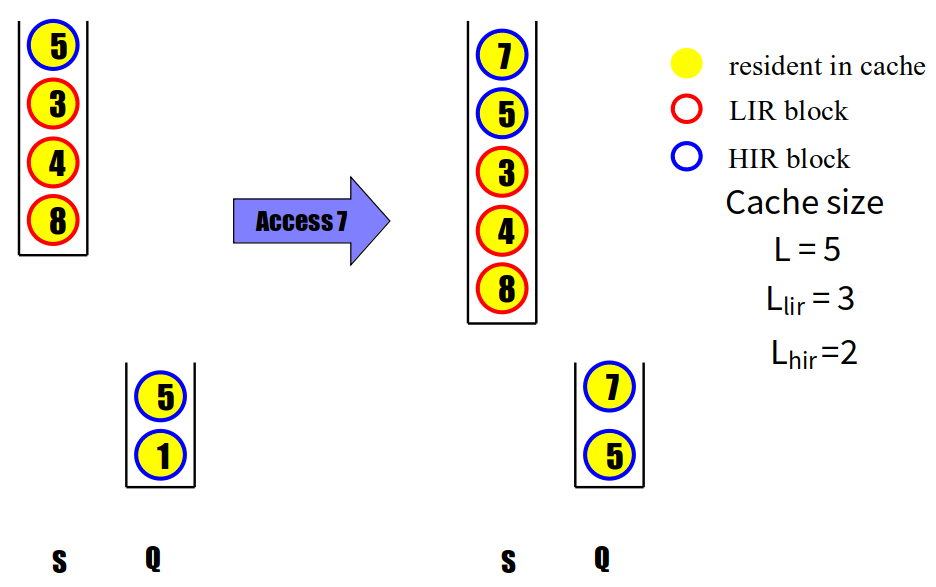
\includegraphics[width=.8\textwidth]{lirs-stack-miss-1}
			
		\end{column}
		
		
	\end{columns}
\end{frame}


%----------------------------------------------
\begin{frame}[plain]
	\frametitle{ }
	\begin{columns}
		\begin{column}{.1\textwidth}
			\centering
			%			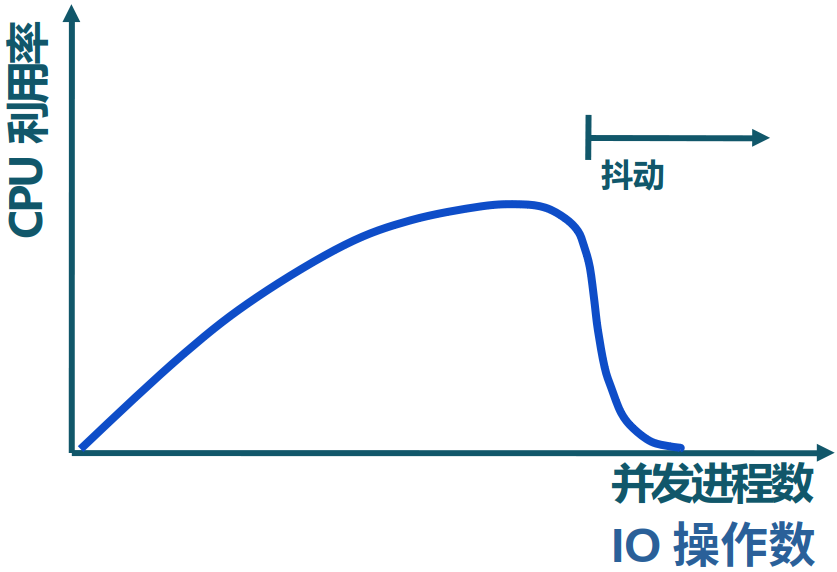
\includegraphics[width=.6\textwidth]{mem-trash}
			
			
		\end{column}
		
		\begin{column}{.9\textwidth}
			LIRS 替换算法 (Missing)
			%			\begin{itemize}
			
			\begin{itemize}
				%				\item 访问栈S中的LIR块X:LIR块必定驻cache中,所以必定命中缓存。然后把块X移动到栈S的头部,如果块X之前是在栈S的底部,则执行“栈裁剪”操作。
				
				%								\item 访问驻cache中的HIR块X:访问命中缓存。把X移动到栈S头部。另外块X有两种情况:(1)块X在栈S中,把它状态转换为LIR,还删除队列Q中块X的cache。然后把栈S底部的LIR块转换为HIR块,然后移动到队列Q中。最后“栈裁剪”。(2)块X不在栈S中,则块X的状态保持HIR不变,然后从队列Q的cache移动到队列尾部。
				%				
				\item 访问非驻留的HIR块X。删除Q尾部的HIR块,如果该块在栈S,则变为非驻留状态,加载块X,把X移动到栈S的顶部。有两种情况:
				\begin{itemize}
				 \item 块X在栈S中,改变状态为LIR,并同时改变栈底部的LIR块为HIR块,并移动到队列Q的头部,然后“栈裁剪”。
%					\item 块X不在栈S中,则状态为HIR,并放到队列Q的头部。
					
					
				\end{itemize}
			\end{itemize}
			\centering
			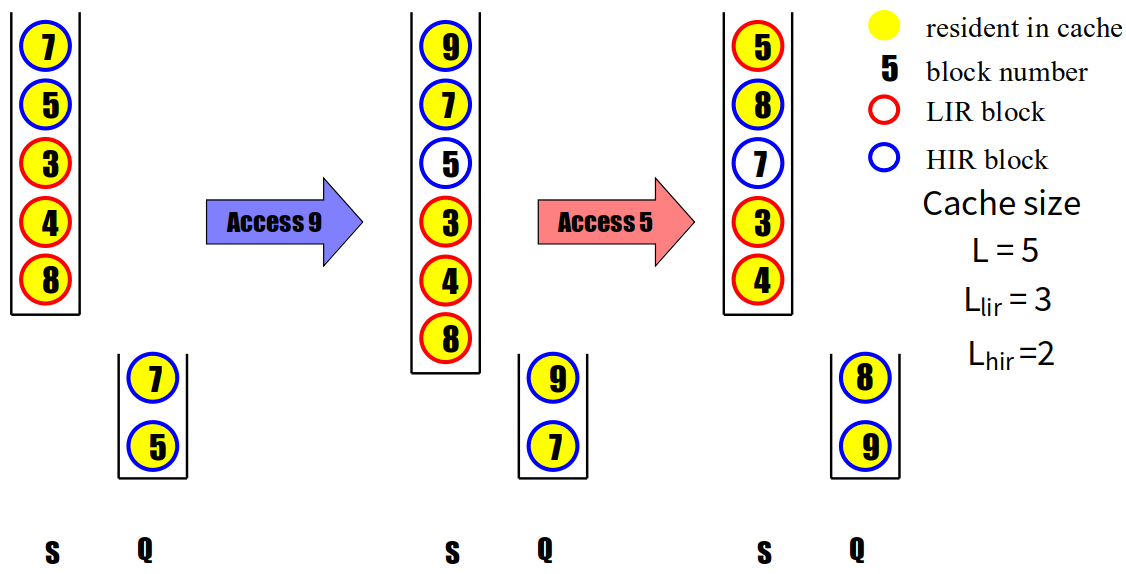
\includegraphics[width=.8\textwidth]{lirs-stack-missing-2}
			
		\end{column}
		
		
	\end{columns}
\end{frame}


%----------------------------------------------
\begin{frame}[plain]
	\frametitle{ }
	\begin{columns}
		\begin{column}{.3\textwidth}
			\centering
			%			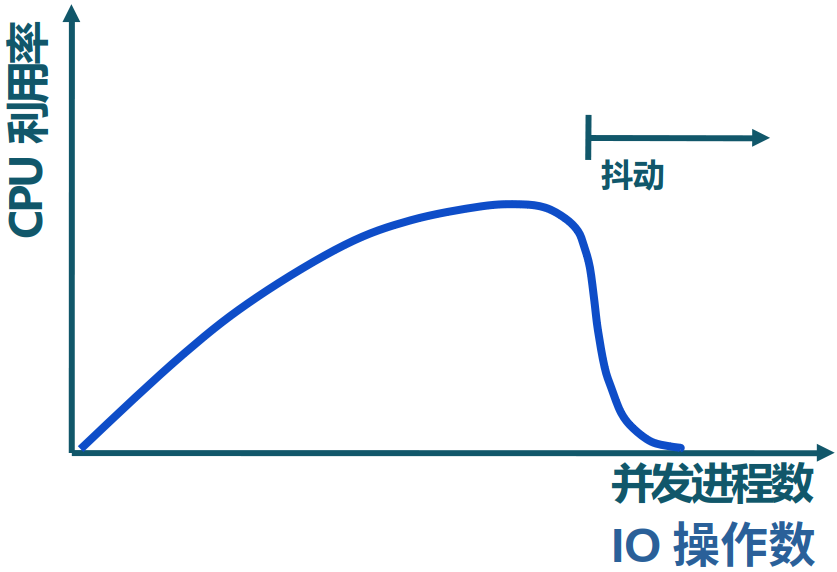
\includegraphics[width=.6\textwidth]{mem-trash}
			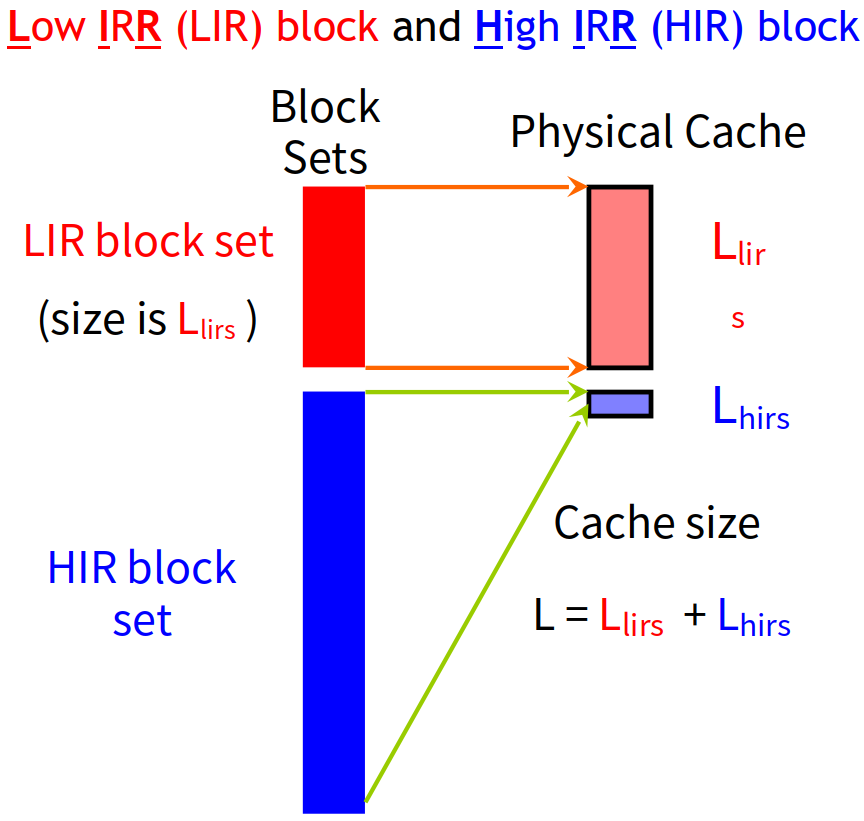
\includegraphics[width=.8\textwidth]{lirs}
			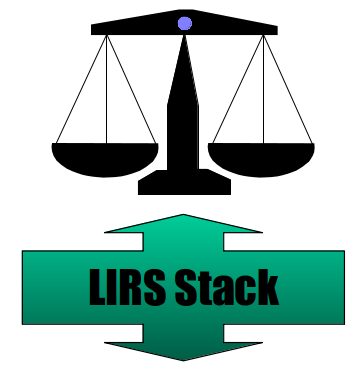
\includegraphics[width=.6\textwidth]{lirs-balance}
		\end{column}
		
		\begin{column}{.6\textwidth}
			
			\begin{itemize}
				\item 评价LIRS
				\begin{itemize}
					\item LIRS能够快速适应上述4种访问模式。
					\item 特别对于循环访问,LIRS能够固定开始的LIR块驻cache中,保证了cache命中率。
					\item LIRS不像2Q等需要设置过多参数。
					\item 实现的复杂度类似LRU。
					\item  从性能角度来看,LIRS>2Q>LRU-K>LRU
					
				\end{itemize}
			\end{itemize}
			\centering
			\large 从能否进一步改进?(Your Work)
			
		\end{column}
		
		
	\end{columns}
\end{frame}

%----------------------------------------------------------------------------------------

\end{document}
